\chapter{Types of NoSQL databases}
\noindent Structured Query Language, or SQL, was developed by IBM following \textcite{coddRelationalModelData1970}'s groundbreaking 
publication in the ACM journal, with the first commercial SQL implementation being published by Oracle in 1979 \autocite{oracleHistorySQL}.
SQL powers many relational database systems even today, though the problems associated with its age, most notably in 
the speed of its operations, are beginning to show in modern systems. Therefore, NoSQL ("Not Only SQL") was developed as 
an extension of SQL, allowing data to be stored in a non-tabular, non-relational format for efficient storage of
semi-structured and unstructured data in a flexible, functional and scalable model for faster operations than standard 
relational databases in most scenarios \autocite{googlecloudWhatNoSQLDatabases, awsWhatNoSQLDatabase}. 

\para There are a wide variety of NoSQL database types - all of which vary in complexity, functionality and purpose, meaning that the
identification of the most suitable type is paramount for maximum efficiency in terms of speed, storage and scalability. 


\section{Document database}\label{sec:DocDBs}
% ? MongoDB is a document database.
% * General purpose databases.
Document databases are intuitive, flexible and horizontally scalable databases that work well in a wide variety of use cases
for both transactional and analytical purposes, including IoT data and real-time analytics \autocite{mongodbDocumentDatabaseNoSQL}.
They store records as "documents", which store an object's data and metadata, in a format such as JSON, BSON, or XML\footnote{JavaScript Object Notation, Binary JSON and Extensible Markup Language, respectively.}. Details and examples of these file types can be found in Appendix A.

% TODO: Finish Appendix A, where you talk about and give examples of each of these. See Lab 4 slides for modelling relationships with JSON.

\begin{figure}[H]
    \centering  
    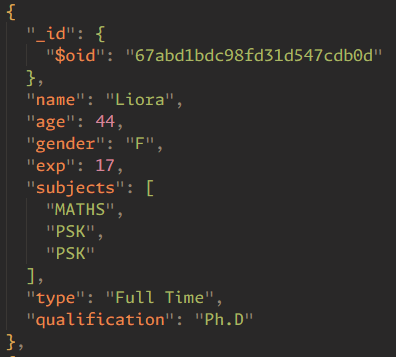
\includegraphics[width=0.6\textwidth]{NoSQL DBs/Doc/ExampleDoc}
    \caption{An example of a JSON Document.\label{fig:ExampleDoc}}
\end{figure}

\noindent Figure \ref{fig:ExampleDoc} depicts an example JSON document in MongoDB\footnote{MongoDB actually stores data as BSON, though it translates between the two when queried. See Appendix B for more information.}, a popular DBMS
for document databases. It contains the data of a singular example school teacher, storing details such as their name, age and subject expertise, as well as a unique internal object ID used by MongoDB to identify that document. The data itself is of varying types including 
strings, integers and arrays, which makes document databases easily integrable into a development workflow due to the direct 
storage of object types used in programming languages like Python and JavaScript.

\para Relationships in document databases can be modelled with great ease, with the ability for documents to contain other documents. 
For example, in MongoDB, a document for a social media user may contain the Object ID of each of their posts. Groups of documents can then
be stored in \textbf{collections}, similar to tables in relational databases. These collections can be queried to perform all CRUD operations. 

% TODO: Talk more about collections and relationship handling.

\para Popular services for document databases include Databricks \autocite{databricksDataAICompany2023} Couchbase \autocite{couchbaseCouchbaseBestFree}, and the previously mentioned MongoDB \autocite{mongodbDocumentDatabaseNoSQL}.


\section{Key-value database}
% ? Redis is a key-value database.
% ! While that's true, it's also an in-memory database.
% * Very fast, very simple.
Key-value databases are primarily reputed for their speed and simplicity, functioning by storing each record as a key-value pair.
Rather than having to search through massive amounts of irrelevant data for a query, key-value databases can instead search 
through their stored keys to retrieve results within milliseconds or even microseconds if used in-memory \autocite{redisRedisFAQ}.
While this is excellent for simple queries to retrieve specific known records, this same property also causes major limitations in
that retrieving data based on values, such as finding all users over a given age, would require the entire database to be searched,
making key-value databases best suited for real-time data access and caching where simpler queries are used \autocite{mongodbWhatKeyValueDatabase}.

% TODO: You've spoke of key-value negatives here, so go back and do it for documents too.

\begin{figure}[H]
    \centering
    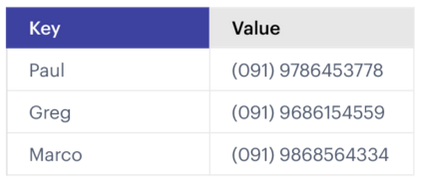
\includegraphics[width=0.5\textwidth]{NoSQL DBs/KeyValue/ExampleKeyVal}
    \caption{An example key-value pair \autocite{redisWhatKeyValueDatabase}.\label{fig:ExampleKeyVal}}
\end{figure}


\noindent Figure \ref{fig:ExampleKeyVal} depicts an example key-value pair, mapping names to phone numbers. If a query for "Greg" was given, 
the associated value would be returned. There is a significant similarity between key-value stores and document stores, though key-value stores
can only store simple key-value pairs, whereas document stores can have flexible schemas of complex, nested structures. Furthermore, as previously 
mentioned, querying key-value databases is very limited to only simple queries if speed is a decisive factor. 

\para Notable software options used across industry for key-value databases include Amazon's DynamoDB \autocite{awsFastNoSQLKeyValue}, Redis \autocite{redisWhatKeyValueDatabase}, and Memcached \autocite{memcachedMemcachedDistributedMemory}. MongoDB can also be used as a key-value store,
though it is not primarily intended to do so.


\section{Wide-column database}
% * Builds on key-value DBs. Stated to have "2 dimensions" which makes sense as it's many values (col groups) to a key I guess?
% ! This is by far the type I know the least. Researching it doesn't seem to really help. Perhaps ask Konstantinos.
% ? Also known as wide-column stores, which may be the preferred term for the module spec.

Wide-column databases, also known as wide-column stores, store data across columns rather than rows, which allows for data schemas built for these 
databases to be very flexible. Records stored in wide-column stores do not require the same columns for every row, which can greatly help to reduce 
duplication and redundancy, and storage requirements by extension. Instead, Figure \ref{fig:ExampleWideCol} depicts how wide-column databases can store 
data in "column groups", which would be defined when the database is created.

\begin{figure}[H]
    \centering
    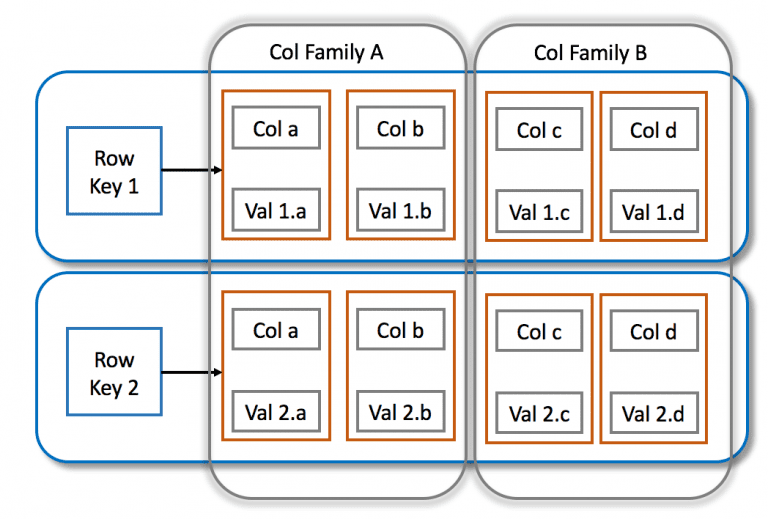
\includegraphics[width=0.5\textwidth]{NoSQL DBs/Column/WideColGroups}
    \caption{An example of wide-column store groups \autocite{poreNoSQLDataArchitecture2018}.\label{fig:ExampleWideCol}}
\end{figure}

\noindent Column groups are greatly beneficial for \textbf{distributed databases}, which leverage sharding for horizontal scalability, a concept
explored further in Chapter 2.
For example, one node could store the columns of group A, whereas another stores group B. If done correctly, this can greatly help the speed
of queries on the database, but it could also cause major slowdowns if the column groups are incorrectly defined, such as with data that would
typically be queried together being split over multiple column groups. Therefore, column groups should consist of data that is frequently 
queried together, such as a group for personal information, then another for financial information \autocite{cattellScalableSQLNoSQL2011}. 

% ! Should you have already spoken about sharding before this point?

\para Because of this, wide-column stores are typically used for larger databases reaching petabytes in size, using software implementations such
as Google's Bigtable \autocite{changBigtableDistributedStorage2008} and Apache Cassandra \autocite{apacheApacheCassandraApache}.


\pagebreak

\section{Graph database}
% ? Neo4J is a graph database.
Graph databases differ heavily from the previously mentioned types, and are instead based on mathematical graph theory \autocite{awsWhatGraphDatabase}.
Rather than storing data as rows and columns (or keys and values), these 
databases store data as nodes and edges. Nodes are connected through their relationships to other nodes, which form the edges of the graph 
structure as depicted in Figure \ref{fig:ExampleGraph}.

\begin{figure}[H]
    \centering
    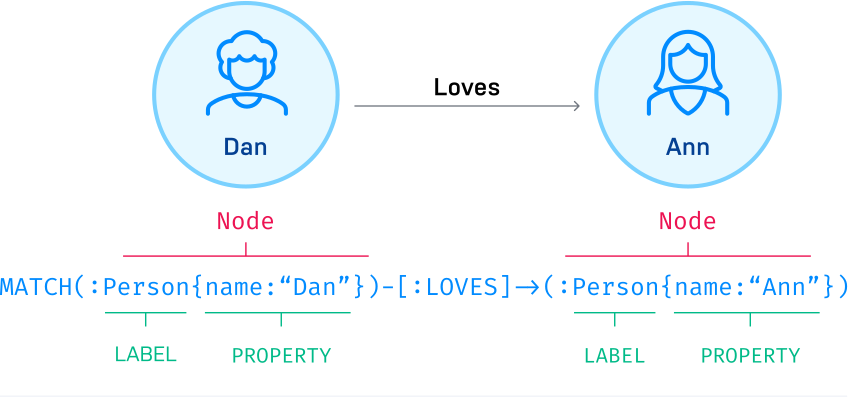
\includegraphics[width=0.5\textwidth]{NoSQL DBs/Graph/ExampleGraph}
    \caption{Two example nodes connected by a relationship. \autocite{neo4jWhatGraphDatabase}\label{fig:ExampleGraph}}
\end{figure}

\noindent Graph databases are best suited for data that is highly interconnected, and can achieve extremely fast query speeds in these scenarios
due to graph traversal, where related nodes can be immediately read through the relationships between them rather than the extensive joins
that would be required in a relational database equivalent \autocite{corbelliniPersistingBigdataNoSQL2017}. Typical use-cases of these 
databases include fraud detection, user recommendation systems and identity management \autocite{neo4jGraphDatabaseUse,awsManagedGraphDatabase,memgraphGraphDatabaseVs}.

\para Software typically used for graph databases includes Neo4J \autocite{neo4jNeo4jGraphDatabase2025}, Amazon 
Neptune \autocite{awsManagedGraphDatabase}, and Memgraph \autocite{memgraphMemgraphDatabase}.

\para An additional key feature of graph databases is that they do not store collections of data together in groups or collections 
unlike other databases, with this functionality instead being dictated by labels, relationships or properties. 

\subsubsection{Label grouping}
Nodes can be labelled with a tag (such as "User"), and queries can instead retrieve all nodes sharing a given label.

\subsubsection{Relationship grouping}
A node is created that represents the group, with all members of the group having a relationship with this parent node such as "Member of".

\subsubsection{Property grouping}
Nodes individually store a property such as a group ID which identifies their particular group. Queries can then fetch all nodes with the given 
property to identify members of the group.

\section{The CAP theorem}
% TODO: Talk about the CAP theorem:
% ?     Consistency: Once data is written, it is available to all users of the system immediately.
% ?     Availability: The service is uninterrupted and without degradation for the majority of the time.
% ?     Partition Tolerance: Operations can be completed even if part of the network fails.
% * It's said that a distributed system can only ever achieve two of these.
% * https://www.ibm.com/think/topics/cap-theorem
The CAP theorem \autocite{brewerRobustDistributedSystems2000} is a foundational governing principle of all distributed systems. He stated that any 
system that shares data across devices can only ever have two of the following three properties:

\begin{longtable}{ | p{0.3\textwidth} | p{0.6\textwidth} | }
    \hline
    \cellcolor{blue!25}Property & \cellcolor{blue!25}Description\\
    \hline
    Consistency & All clients see the same data at the same time, irrespective of the node they're connected to.\\
    \hline
    Availability & A response is always given to a client request, even if a node (or multiple) is down.\\
    \hline
    Partition Tolerance & The system must continue to operate even if nodes temporarily lose connection to each other.\\
    \hline
    \caption{The properties of the CAP theorem. \autocite{brewerRobustDistributedSystems2000,ibmWhatCAPTheorem2022}}\label{tab:CAPTheorem}
\end{longtable}

\noindent The CAP theorem is vitally important in the selection of which NoSQL database type to use, as different DBMS adhere to different 
properties of the theorem, with none being able to offer all three as stated by Brewer. 

\para For example, the document database MongoDB adheres to Consistency and Partition Tolerance (CP), but is unable to 
offer total availability because of this. This is because ensuring CP means that data between nodes cannot be inconsistent, so if nodes fail to 
synchronise data, the availability would have to suffer to stop potentially outdated data being returned.

\para Another example is the wide-column store Apache Cassandra, which offers Availability and Partition Tolerance (AP), but 
therefore cannot offer total consistency. Cassandra instead offers "eventual consistency" through the BASE transactional model, which is 
described in Section \ref{subsec:BASE}, where clients can potentially see outdated data during simultaneous queries, though the DBMS aims 
to resolve inconsistencies as quickly as possible.

\para \textcite{ibmWhatCAPTheorem2022} write that consistency and availability (CA) cannot exist simultaneously in 
NoSQL distributed systems, as this would come at the expense of Partition Tolerance which is not possible in a distributed system. 
Instead, a relational database would have to be used to offer both of these.

% ! I don't know where it'd be best to talk about the CAP theorem.
% ! I'm not massively happy with some of the explanations in this chapter as I feel they can be vague or perhaps even outright wrong.
% ! It's not a huge issue, as I believe this area is ~20% of the assignment's grade, with the actual MongoDB part being the majority.